\begin{center}
    \section*{\fontsize{20}{20}\selectfont Chapter 5}
\end{center}
\vspace{10mm}

\section{Standards, Constraints, and Milestones}

The earlier chapters showed that the plant disease detection system can be built and how well it performs. It is just as important to look at the system from other sides: engineering standards, its effect on society and ethics. In this chapter we list the standards we followed, look at how this technology may affect farming and society, and discuss the ethical duties that come with using AI in real life. We also describe the technical problems we faced and the limits of this work.

\subsection{Sustainability Standards}
The project supports the United Nations Sustainable Development Goals (SDGs), and it follows some basic software and testing standards.

\subsubsection*{Alignment with UN Sustainable Development Goals (SDGs)}
Automatic crop disease screening that can explain itself supports farming in a sustainable way. Table~\ref{tab:sdg_alignment} shows how it links to five UN SDGs.

\begin{table}[htbp]
\caption{Alignment of the Proposed System with UN Sustainable Development Goals}
\label{tab:sdg_alignment}
\begin{center}
\begin{tabularx}{\textwidth}{| p{2.3cm} | p{3.6cm} | X |}
\hline
\textbf{UN SDG} & \textbf{Goal Title} & \textbf{How the Project Helps} \\
\hline
SDG 2 & Zero Hunger & Early diagnosis of potato diseases in the field (such as late blight caused by \textit{Phytophthora infestans}, and fungal, bacterial and viral infections) helps small farmers lose less of their crop and improves food security. \\
\hline
SDG 9 & Industry, Innovation, and Infrastructure & A compact MobileNetV2 model (2.26M parameters, 8.64~MB) runs fast on low-cost servers and is ready for offline smartphones, and the open-source pipeline can be repeated by anyone. \\
\hline
SDG 12 & Responsible Consumption and Production & Finding the exact disease, together with safe LLM advice, helps farmers avoid spraying the whole field. They waste less chemical and use their inputs better. \\
\hline
SDG 13 & Climate Action & Farmers can react fast when the changing climate brings new pest and disease outbreaks, and less chemical is made and washed into the fields. \\
\hline
SDG 15 & Life on Land & Using less fungicide and pesticide protects soil life, bees and the water near the fields. \\
\hline
\end{tabularx}
\end{center}
\end{table}

\subsubsection*{Engineering and Software Standards}
We also followed engineering and testing standards during the whole project.

\textit{Coding standard (PEP 8).} All code is written in Python and follows the PEP~8 style guide. Indentation is consistent, function names use \texttt{snake\_case} and class names use \texttt{CamelCase}, so the code is easy to read and maintain.

\textit{Data license.} The dataset comes from a public Kaggle repository. We use it only for study and research, as the authors' license allows \cite{shabrina2024novel}.

\textit{Testing standard.} We used standard machine learning metrics: accuracy, precision, recall, macro and weighted F1-score and confusion matrices. They were computed on a 10\% leak-aware test split ($N = 231$) that was kept apart from training, with a fixed random seed ($42$), so the results can be repeated \cite{grandini2020metrics}.

\subsection{Impacts on Society}
An automatic plant disease detector can affect society in several ways, especially in farming.

\textit{Food security.} Finding potato problems early, such as Phytopthora (late blight), fungal and bacterial diseases, viruses and pests, can stop large crop losses. This supports SDG 2: Zero Hunger.

\textit{Saving money for farmers.} In many developing areas, farmers must pay expensive experts or simply guess, and a wrong guess can ruin the crop. Once the system is accurate enough, it can give a cheap first diagnosis and simple advice through the LLM module. This lowers costs and prevents losses.

\textit{Protecting the environment.} A wrong diagnosis often leads to spraying too much pesticide everywhere. If farmers know the exact disease, they can treat only what is needed (precision agriculture). Less chemical then runs into the soil and water, which protects nature.

\subsection{Ethics}
Using AI in farming brings some ethical duties. We dealt with them as follows.

\textit{Bias in the data.} The classes are somewhat uneven (729 Fungi images against 199 Healthy images). To lower this risk we used a leak-aware grouped split, data augmentation and class weights during training, and selected checkpoints by macro-F1.

\textit{Risk of a wrong diagnosis (false negatives).} If we tell a farmer that a sick plant is healthy, or name the wrong disease, the farmer may lose the crop. We used label smoothing so the model is less over-confident, show Grad-CAM overlays for visual checking, and display a clear reminder that the AI gives screening support rather than a final lab diagnosis.

\textit{Privacy and careful use of the LLM.} The dataset has no personal data. The Gemini API key is kept in environment secrets, not in the code. Only the predicted class and the confidence are sent to the LLM, not the image, and the prompt does not allow made-up pesticide doses.

\subsection{Challenges}
We met three big problems during the research.

\textit{Uneven classes and near-duplicate photos.} Healthy leaves make up only 8.6\% of the dataset, and field photos often contain burst shots of the same leaf. Grouping near-duplicates with perceptual hashing ($\text{dHash} \le 10$) and using class weights solved both problems.

\textit{Busy backgrounds and similar symptoms.} The photos show soil, hands, plastic mulch and other plants. Different diseases, for example Fungi and Phytophthora, can also show similar brown lesions. This makes the task much harder than with lab datasets.

\textit{Fine-tuning stability on a medium dataset.} Unfreezing Batch Normalization layers during fine-tuning caused a sharp validation-loss spike in our early run. Keeping Batch Normalization frozen in Stage~2 with AdamW removed the spike and lifted accuracy from 91.34\% to 93.51\%.

\subsection{Constraints}
Every research project has practical limits on technology, parts and money. Our main limits were these.

\textit{Design limits.} The model takes a fixed $224 \times 224 \times 3$ RGB input. Our proposed MobileNetV2 had to stay under 10~MB (8.64~MB weights) and expose its final convolutional layer (\texttt{Conv\_1}) for Grad-CAM. It classifies 5 potato leaf classes, and the LLM prompt forbids invented doses.

\textit{Component limits.} The dataset has 2,321 field images (with 19 Healthy test samples), so a few mild fungal false positives still lower Healthy precision to 0.79. Also, the advice module needs the outside Google Gemini API and an internet connection, which can be unstable in rural farm areas.

\textit{Budget limits.} This was a student capstone project with no outside funding. We used only free Kaggle dual-T4 GPU quotas and open-source software, and called \texttt{gemini-3.1-flash-lite} once per request to stay within low-cost API limits.

\textit{Operational and legal limits.} Even at 93.51\% accuracy, AI screening is not a replacement for certified plant pathologists. Our web interface clearly marks every result as preliminary guidance and advises consulting local agricultural officers when uncertain.

\subsection{Timeline and Gantt Chart}
We had six months to finish this research, so we made a clear work plan. The project had two phases: Phase I (planning and design) and Phase II (building and analysis). Figure~\ref{fig:gantt1} and Figure~\ref{fig:gantt2} show the tasks and their timing as Gantt charts.

\subsubsection{Phase I: Planning and System Design (Weeks 1--13)}
In the first phase we studied the background and prepared what we needed for the experiment. As Figure~\ref{fig:gantt1} shows, this phase took the first three months (Weeks 1 to 13):
\begin{itemize}
    \item \textbf{Weeks 1--2:} We read earlier studies to find the gaps in current plant disease detection methods.
    \item \textbf{Weeks 3--5:} We collected the Potato Leaf Disease (Uncontrolled Environment) dataset and explored it (EDA) to understand the class counts.
    \item \textbf{Weeks 6--10:} We designed our Proposed MobileNetV2 model and set up the leak-aware split, normalization and augmentation.
    \item \textbf{Weeks 11--13:} We chose and set up the benchmark models (MultiNet-V3 Ensemble and InceptionV3) and finished the research method.
\end{itemize}

\begin{figure}[htbp]
\centering
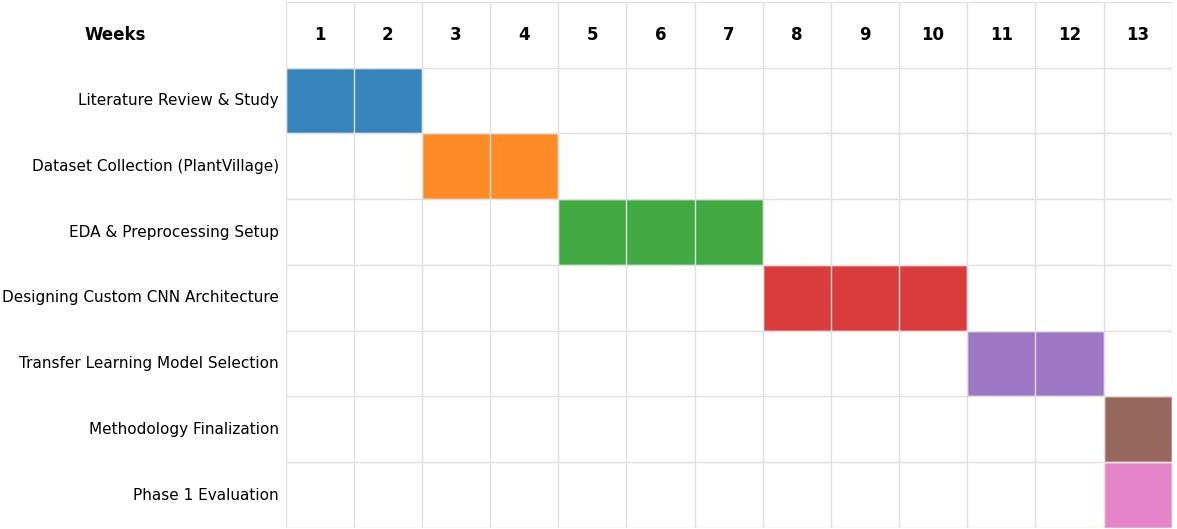
\includegraphics[width=0.95\textwidth]{image/docx_image26.jpeg}
\caption{Gantt Chart I -- Timeline for Planning, Data Preparation, and Model Design (Weeks 1--13).}
\label{fig:gantt1}
\end{figure}

\subsubsection{Phase II: Implementation, Testing, and Documentation (Weeks 14--26)}
In the second phase we built and tested the system and wrote up the results. As Figure~\ref{fig:gantt2} shows, this phase took the last three months (Weeks 14 to 26):
\begin{itemize}
    \item \textbf{Weeks 14--17:} We trained the three models (Proposed MobileNetV2, MultiNet-V3 Ensemble and InceptionV3) on Kaggle dual T4 GPUs and tuned them to improve accuracy.
    \item \textbf{Weeks 18--21:} We compared the models by accuracy, loss, F1-score and model size. We also built the Explainable AI part (Grad-CAM), the Gemini LLM advice module and the live web application.
    \item \textbf{Weeks 22--26:} We finished the results, plotted the metrics (confusion matrices, comparison charts) and wrote the full thesis. At the end, we prepared for the final defense presentation.
\end{itemize}

\begin{figure}[htbp]
\centering
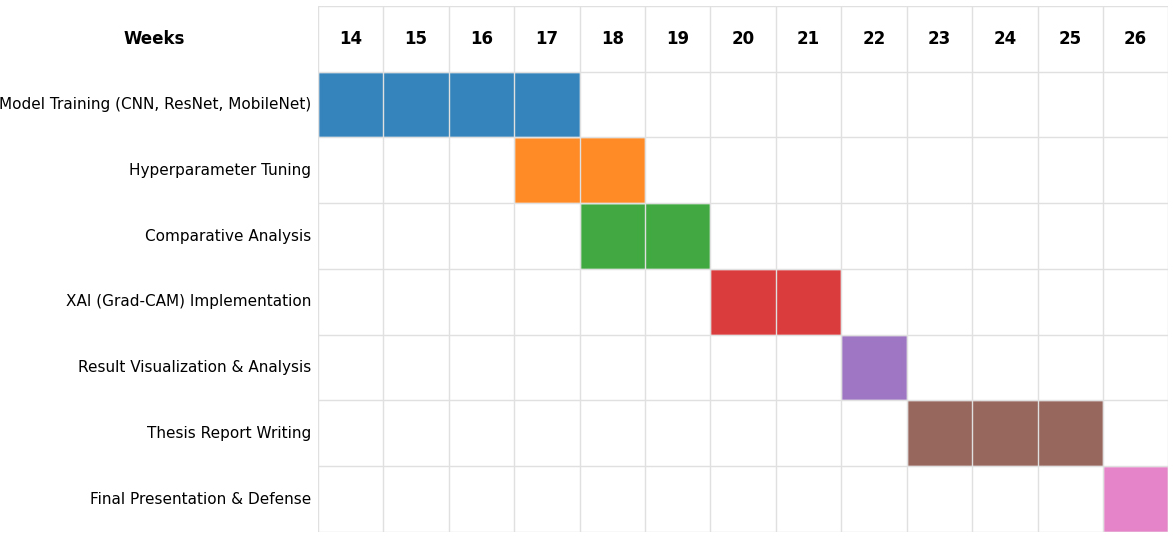
\includegraphics[width=0.95\textwidth]{image/docx_image27.png}
\caption{Gantt Chart II -- Timeline for Implementation, Testing, and Final Documentation (Weeks 14--26).}
\label{fig:gantt2}
\end{figure}
